% =====================================================================
%  SKELETON / DRAFT — GPU-accelerated differentiable DTL reconciliation
%  Experiments are left as clearly marked placeholders (see \expbox).
%  Compiles with: pdflatex gpurec_paper.tex  (run twice for refs)
% =====================================================================
\documentclass[11pt]{article}

\usepackage[utf8]{inputenc}
\usepackage[T1]{fontenc}
\usepackage{amsmath,amssymb,amsthm}
\usepackage{graphicx}
\graphicspath{{figures/}}
\usepackage{booktabs}
\usepackage{xcolor}
\usepackage[margin=1in]{geometry}
\usepackage{microtype}
\usepackage[round,authoryear]{natbib}
\usepackage[colorlinks=true,allcolors=blue]{hyperref}
\usepackage{enumitem}
\usepackage{xspace}

% ---- tool name (change in one place) -------------------------------
\newcommand{\toolname}{\textsc{gpurec}\xspace}

% ---- experiment placeholder box ------------------------------------
% Use \begin{expbox}{short title} ... \end{expbox} to mark a hole and
% describe WHAT the experiment must demonstrate.
\newenvironment{expbox}[1]{%
  \par\smallskip\noindent
  \begin{center}\begin{minipage}{0.96\linewidth}\small
  \rule{\linewidth}{0.8pt}\par
  \textbf{\color{red!60!black}[EXPERIMENT --- #1]}\par\itshape
}{%
  \par\rule{\linewidth}{0.8pt}
  \end{minipage}\end{center}\smallskip
}
% inline TODO
\newcommand{\TODO}[1]{{\color{red!70!black}\textbf{[TODO: #1]}}}

% ---- math shortcuts ------------------------------------------------
\newcommand{\bdelta}{\delta}
\newcommand{\btau}{\tau}
\newcommand{\blambda}{\lambda}
\newcommand{\NLL}{\mathcal{L}}
\newcommand{\Hess}{\mathbf{H}}
\newcommand{\Fish}{\mathbf{I}}
\newcommand{\grad}{\mathbf{g}}
\newcommand{\Real}{\mathbb{R}}

\title{\textbf{\toolname: A GPU-Accelerated, Differentiable Framework for\\
Gene--Species Tree Reconciliation under the DTL Model\\
\large with Certified Optima, Flexible Priors, and Transfer Heterogeneity}}

\author{%
  \TODO{author list} \\[2pt]
  \small \TODO{affiliations}
}
\date{Draft --- \today}

\begin{document}
\maketitle

% =====================================================================
\begin{abstract}
\noindent
Reconciling gene trees with a species tree under a model of gene
\emph{duplication, transfer, and loss} (DTL) is central to comparative
genomics. Existing reconciliation software --- including the state-of-the-art
\textsc{AleRax} --- treats the amalgamated likelihood as a fixed, hand-%
differentiated black box, optimized by first-order methods on the CPU. We
re-implement the \textsc{UndatedDTL} reconciliation likelihood as a fully
\emph{differentiable} GPU program, exposed through a \textsc{PyTorch} interface.
Our central claim is methodological: \emph{differentiable reconciliation is an
enabling computational paradigm} --- exact gradients, Hessian--vector products,
the information matrix, uncertainty quantification, custom priors, and model
extensions all follow from it, essentially for free. Concretely, this single
capability yields (i) order-of-magnitude faster maximum-likelihood estimation of
per-family (``genewise'') DTL rates; (ii) \emph{second-order} inference ---
certified \emph{local} optimality via the Hessian spectrum, and the observed-%
information matrix for parameter uncertainty and non-identifiability analysis;
(iii) \emph{arbitrary user-defined penalties}, demonstrated by cross-validating a
tree-smoothing prior for species-wise rates on \textsc{Hogenom}, a computation
that would be infeasible on the CPU; and (iv) \emph{per-recipient transfer
weights} that infer which species disproportionately receive horizontal
transfers, relaxing the uniform-recipient assumption and addressing a feature
listed as future work for \textsc{AleRax}. We demonstrate on the
\textsc{Hogenom-Core} and archaeal datasets, and release \toolname as an open,
extensible engine. \TODO{1--2 sentences of headline quantitative results once
experiments land.}
\end{abstract}

% =====================================================================
\section{Introduction}
\label{sec:intro}

Genomes record evolution at multiple scales: substitutions accumulate along
gene trees, while gene duplication, horizontal transfer, and loss reshape gene
family histories relative to the species tree \citep{Szollosi2015}. Accounting
for this discord is the goal of probabilistic \emph{reconciliation} under the
DTL model. Because individual gene trees are themselves uncertain, modern
methods integrate over a \emph{distribution} of gene trees summarised by
conditional clade probabilities (CCPs), as in Amalgamated Likelihood
Estimation \citep{Szollosi2013,Hohna2012,Larget2013}. \textsc{GeneRax}
\citep{Morel2020}, \textsc{SpeciesRax} \citep{Morel2022}, and most recently
\textsc{AleRax} \citep{Morel2024} build on this framework to co-estimate
reconciled gene trees and a shared species tree under the \textsc{UndatedDTL}
model.

\textsc{AleRax} is the current state of the art for amalgamated DTL
reconciliation. It estimates the model's rate parameters --- per branch $e$, a
duplication, transfer, and loss probability
$(\bdelta_e,\btau_e,\blambda_e)$ --- by \emph{gradient descent} on the
amalgamated likelihood, and supports three parameter-sharing regimes:
\emph{global} (all families and branches share $(\bdelta,\btau,\blambda)$,
$3$ parameters), \emph{per-family} ($3K$ parameters for $K$ families), and
\emph{per-species} ($3n$ parameters for $n$ user-defined species groupings)
\citep{Morel2024}. It runs an order of magnitude faster than ALE and scales to
genome-wide datasets with hundreds of taxa.

\paragraph{Why \textsc{AleRax} is our primary baseline.} The amalgamated-DTL
lineage comprises ALE \citep{Szollosi2013}, which scores a fixed species tree
against gene-tree distributions; \textsc{GeneRax} \citep{Morel2020}, which
infers reconciled gene trees from \emph{single} maximum-likelihood gene trees
(no gene-tree-distribution input); \textsc{SpeciesRax} \citep{Morel2022}, which
targets species-tree inference; and \textsc{AleRax} \citep{Morel2024}, which
unifies these by estimating DTL rates and reconciliations from gene-tree
\emph{distributions} with the same per-family/per-species rate-sharing modes we
adopt, an order of magnitude faster than ALE. Because \textsc{AleRax} is the
most recent, fastest, and most directly comparable tool for the
\emph{rate-estimation} task we accelerate --- same likelihood, same
parameter-sharing regimes, same CCP input --- it is the natural head-to-head
baseline; we benchmark against it throughout and reference the others where the
comparison is informative.

Despite these strengths, the rate-estimation engine of existing tools has
structural limitations that motivate this work:
\begin{enumerate}[leftmargin=1.4em,itemsep=2pt]
\item \textbf{First-order, CPU-bound optimization.} Rates are fit with
gradient descent on the CPU. Without curvature information there is no way to
\emph{certify} that an estimate is a (local) optimum, to quantify the
\emph{uncertainty} of the inferred rates, or to detect when parameters are
\emph{non-identifiable} (statistically confounded).
\item \textbf{A fixed model.} The likelihood, recipient distribution for
transfers, and the (absence of a) prior are baked in. Incorporating
biologically motivated structure --- e.g.\ smoothing rates across the species
tree, or letting some lineages be preferential transfer recipients --- is not
readily available to the user. \citet{Morel2024} explicitly list ``DTL rate
heterogeneity over species'' among directions for future work.
\item \textbf{Scale limits on model selection.} Choosing a regularization
strength by cross-validation, or running many restarts, multiplies the cost of
an already expensive fit, which is impractical on the CPU.
\end{enumerate}

\paragraph{Contribution.} We re-implement the \textsc{UndatedDTL} amalgamated
reconciliation likelihood as a differentiable GPU program with a
\textsc{PyTorch} front-end, \toolname. The implementation provides exact
gradients (via implicit differentiation of the model's fixed-point solves) and
exact Hessian--vector products (via forward-over-reverse differentiation),
entirely matrix-free. From this single capability we obtain, without
bespoke derivations:
\begin{enumerate}[leftmargin=1.4em,itemsep=2pt]
\item \textbf{Speed.} GPU evaluation makes per-family rate estimation
embarrassingly parallel across families, giving an order-of-magnitude speedup
over CPU optimization (Sec.~\ref{sec:speed}).
\item \textbf{Certified optima and uncertainty.} Hessian--vector products feed
a Lanczos solver that certifies a positive-definite local minimum, and yield
the Fisher (observed) information matrix for asymptotic confidence intervals
and identifiability analysis (Secs.~\ref{sec:certify}--\ref{sec:fisher}).
\item \textbf{Flexible priors / penalties.} Any differentiable penalty
$R(\theta)$ can be added to the loss; we cross-validate a tree-smoothing prior
for species-wise rates on \textsc{Hogenom} (Sec.~\ref{sec:cv}).
\item \textbf{Transfer heterogeneity.} Learned per-recipient weights identify
species that receive more transfers than others (Sec.~\ref{sec:receiver}).
\end{enumerate}

\paragraph{Scope.} We focus on the \emph{parameter-estimation /
reconciliation-likelihood} component: given a fixed species tree and per-family
CCP distributions, infer DTL rates (and reconciliations). Species-tree search,
as performed by \textsc{SpeciesRax}/\textsc{AleRax}, is orthogonal and could be
driven by the same differentiable engine; we return to this in
Sec.~\ref{sec:discussion}.

% =====================================================================
\section{Model and Methods}
\label{sec:methods}

\subsection{The amalgamated \textsc{UndatedDTL} likelihood}
\label{sec:lik}
Let $S$ be a rooted species tree and, for each gene family $i$, let $A_i$ be a
sample of gene trees summarised by its CCP distribution. Under amalgamation,
the family likelihood marginalises over all gene trees compatible with the CCPs
\citep{Szollosi2013}:
\begin{equation}
  P(A_i \mid S) \;=\; \sum_{G} P(A_i \mid G)\, P(G \mid S),
  \label{eq:amalg}
\end{equation}
and the dataset likelihood factorises over families,
$\mathcal{L}(S \mid A) = \prod_i P(A_i \mid S)$. Under \textsc{UndatedDTL}, a
gene lineage on species-tree branch $e$ undergoes duplication, transfer, and
loss with per-branch probabilities $(\bdelta_e,\btau_e,\blambda_e)$; survival
probabilities are obtained from a fixed-point (``extinction'') equation, and
$P(A_i\mid S)$ from a dynamic-programming recursion over CCP clades
\citep{Szollosi2013,Morel2020}. We collect the free log-rate parameters into a
vector $\theta$ and write the negative log-likelihood
$\NLL(\theta) = -\sum_i \log P(A_i \mid S;\theta)$.

\subsection{Parameter-sharing modes}
\label{sec:modes}
\toolname supports the same sharing regimes as \textsc{AleRax}: \emph{global}
($\theta\in\Real^{3}$), \emph{genewise} (per-family, $\theta\in\Real^{3K}$),
and \emph{specieswise} (per-species or per-grouping, $\theta\in\Real^{3n}$;
$p=3n$). The genewise mode reproduces the per-family optimization of
\textsc{AleRax} and is the natural target for the speed comparison; the
specieswise mode is the setting in which priors and second-order analysis are
most informative.

\subsection{A differentiable GPU implementation}
\label{sec:autodiff}
The likelihood is implemented as a \textsc{PyTorch} tensor program. The two
inner solves --- the extinction fixed point and the per-clade survival/transfer
recursion --- are iterative, and we differentiate them by \emph{implicit
differentiation} rather than by differentiating a truncated unrolled loop.
\emph{Hessian--vector products} $\Hess(\theta)\,v$ are obtained matrix-free by
forward-over-reverse differentiation, so second-order information costs a small
constant number of solves per product and never forms the $p\times p$ Hessian.
Throughput is sustained by batching families across the GPU and, optionally, by
adapting per-batch solver fidelity (the number of fixed-point / Neumann
iterations) to each batch's convergence, so that ``easy'' families are not
over-solved.

\paragraph{Why implicit differentiation is correct.} Let $x^\star(\theta)$ be
the converged solution of the model's fixed-point map,
\begin{equation}
  x^\star(\theta) \;=\; F\!\left(x^\star(\theta),\,\theta\right),
  \label{eq:fixedpoint}
\end{equation}
(the extinction probabilities, and similarly the clade recursion). By the
implicit function theorem, differentiating Eq.~\eqref{eq:fixedpoint} gives
\begin{equation}
  \frac{d x^\star}{d\theta}
   \;=\; \bigl(I-\partial_x F\bigr)^{-1}\,\partial_\theta F ,
  \label{eq:ift}
\end{equation}
valid wherever $\bigl(I-\partial_x F\bigr)$ is invertible (guaranteed when the
fixed-point iteration is contractive, i.e.\ the spectral radius of
$\partial_x F$ is below one --- the same condition under which the forward solve
converges). The downstream loss gradient is then assembled by the chain rule.
Crucially, the inverse in Eq.~\eqref{eq:ift} is \emph{never formed}: the
adjoint/cotangent system $\bigl(I-\partial_x F\bigr)^{\!\top} u = b$ is solved
\emph{iteratively} by a Neumann series (equivalently, the same contraction run
in reverse), so the gradient is exact up to the adjoint solver's tolerance and
costs $O(1)$ extra solves. Differentiating the unrolled forward iterations would
instead make the gradient's accuracy hostage to the (truncated) iteration count
and inflate memory with the full iteration trace; implicit differentiation
decouples gradient accuracy from forward-iteration depth.
\TODO{cite the implicit function theorem / adjoint method; one sentence on the
Triton kernels / Rust preprocessing if desired.}

\subsection{Per-recipient transfer weights}
\label{sec:rweights}
In the standard model a transferred copy is received by a branch drawn from a
fixed, effectively uniform recipient distribution. We relax this with
\emph{species-specific} recipient weights. Let $\alpha\in\Real^{S}$ be a vector
of per-species logits and define the recipient distribution by a softmax,
\begin{equation}
  w_s \;=\; P(\text{recipient}=s) \;=\;
   \frac{\exp(\alpha_s)}{\sum_{r}\exp(\alpha_r)},
   \qquad \textstyle\sum_s w_s = 1 .
  \label{eq:rweights}
\end{equation}
The simplex constraint $\sum_s w_s=1$ removes the scale ambiguity (only relative
weights are meaningful) and makes $w$ \emph{identifiable separately from the
transfer rate} $\btau$: $\btau$ sets the \emph{total} probability that a lineage
is transferred, while $w$ sets only the \emph{normalized distribution} over
recipients. Large $w_s$ flags species that act as transfer \emph{sinks}. Because
$\alpha$ is weakly constrained when transfers into a clade are rare, we
regularize it with a smoothness/entropy prior (e.g.\ the same tree-Laplacian of
Sec.~\ref{sec:penalty} applied to $\alpha$, or a symmetric Dirichlet on $w$),
selected like any other penalty (Sec.~\ref{sec:penalty}). This is a concrete
form of the across-species heterogeneity that \citet{Morel2024} list as future
work.

Because $\alpha$ enters the likelihood only through the softmax of
Eq.~\eqref{eq:rweights}, the loss is exactly invariant under
$\alpha\!\mapsto\!\alpha+c\mathbf{1}$ (a shift of all logits); we fix this gauge
by optimizing in the mean-zero subspace. The receiver-weight analogue of the
rate box of Sec.~\ref{sec:certify} is a floor on the recipient \emph{probability}
itself --- a bound on the logits would be vacuous, since the same softmax shift
that fixes the gauge can drive any $w_s\!\to\!0$ regardless of where the logits
sit. We therefore reparametrize
$w = c\,\mathbf{1} + (1-Sc)\,\mathrm{softmax}(\beta)$ with $c=1/(100S)$, which
guarantees $w_s\!\ge\!1/(100S)$ for every species (no recipient weight collapses)
while leaving dominant transfer sinks ($w_s\!\to\!1$) unconstrained, and optimize
the unconstrained $\beta$. The exact gradient $\partial\NLL/\partial\alpha$ is
produced by the \emph{same} analytic backward that yields the rate gradient (the
recipient distribution is just another differentiable input to the likelihood),
and the matrix-free HVP extends to the full $(\theta,\alpha)$ block. Gradient,
$(\theta,\alpha)$ HVP, and the gauge-projected Fisher information are validated
against \texttt{fp64} finite differences (per-block relative error
$\sim\!10^{-6}$), so $\alpha$ is estimated jointly with the rates and its
identifiability and standard errors come from the same matrix-free machinery, at
no extra derivation cost.

\subsection{Penalized likelihood and priors}
\label{sec:penalty}
Because the objective is an ordinary differentiable function in
\textsc{PyTorch}, the user may add \emph{any} differentiable penalty
$R(\theta)$ and optimize
\begin{equation}
  F_\kappa(\theta) \;=\; \NLL(\theta) \;+\; \kappa\, R(\theta),
  \label{eq:penalized}
\end{equation}
recovering MAP estimation when $\kappa R$ is the negative log-prior. We
highlight two:
\begin{itemize}[leftmargin=1.4em,itemsep=2pt]
\item \textbf{Ridge / Gaussian prior:} $R(\theta)=\tfrac12\|\theta-\theta_0\|^2$.
\item \textbf{Tree-smoothing (roughness) prior} in the spirit of
\citet{Sanderson2002}: penalise how much species-wise rates change between
adjacent species-tree branches,
\begin{equation}
  R(\theta) \;=\; \tfrac12 \sum_{(c,p)\in E(S)} \lVert \theta_c - \theta_p \rVert^2 ,
  \label{eq:gbm}
\end{equation}
the quadratic form of a tree graph-Laplacian. This shares statistical strength
across the species tree and regularises otherwise weakly-identified per-species
rates.
\end{itemize}
The penalty strength $\kappa$ is a hyperparameter selected by cross-validation
(Sec.~\ref{sec:cv}).

\subsection{Second-order inference}
\label{sec:second}
At a candidate estimate $\hat\theta$ with gradient $\grad=\nabla F(\hat\theta)$
and Hessian $\Hess=\nabla^2 F(\hat\theta)$ (both available matrix-free):
\begin{itemize}[leftmargin=1.4em,itemsep=2pt]
\item \textbf{Certification.} $\hat\theta$ is a local minimum if
$\|\grad\|\approx 0$ and $\Hess\succ 0$. We estimate the smallest eigenvalue
$\lambda_{\min}(\Hess)$ by Lanczos iteration on the HVP operator; a negative
$\lambda_{\min}$ exhibits a descent (saddle) direction, and a positive
$\lambda_{\min}$ certifies a strict local minimum. When $\lambda_{\min}$ is
near zero we additionally use a true-loss line search along the lowest-curvature
directions as an operational convergence test.
\item \textbf{Information and uncertainty.} We use the \emph{observed
information} matrix --- the Hessian of the negative log-likelihood at the
optimum, $\Fish_{\mathrm{obs}} = \Hess(\hat\theta)$ --- as the standard
large-sample approximation to the Fisher information. (The observed information
and the expected Fisher information $\Fish_F = \mathbb{E}[-\nabla^2\log L]$
coincide asymptotically under the usual regularity conditions but are not
literally equal; we report the observed information, which is what the
matrix-free Hessian gives directly.) Its inverse $\Fish_{\mathrm{obs}}^{-1}$ is
the asymptotic covariance of the rate estimates; diagonal entries give standard
errors / confidence intervals, and the eigenvectors of near-zero eigenvalues
expose \emph{confounded} parameter combinations (non-identifiability).
\item \textbf{Optimization.} The same HVPs drive Newton / trust-region steps
and saddle-escape for the hardest (near-singular) fits.
\end{itemize}

\subsection{Optimization pipeline}
\label{sec:pipeline}
A typical fit runs first-order optimization (Adam) to enter the basin, then a
quasi-Newton phase (L-BFGS), and --- where certification is desired --- a
matrix-free Newton / saddle-escape phase using the HVPs of
Sec.~\ref{sec:second}. Convergence is judged on the projected gradient and,
near singular optima, on the operational line-search criterion.
\TODO{final wording once the specieswise endgame experiment is settled.}

% =====================================================================
\section{Results}
\label{sec:results}

\noindent\emph{Datasets.} We use the empirical datasets of
\citet{Morel2024}: the \textsc{Hogenom-Core} set of $666$ representative
genomes \citep{Penel2009}, from which we draw $1{,}055$ gene families for the
cross-validation study (Sec.~\ref{sec:cv}), and the archaeal dataset of
$5{,}446$ gene families ($\geq\!4$ sequences each) over $S{=}119$ species
spanning DPANN, Euryarchaeota, TACK, and Asgardarchaeota
\citep{Williams2017,Davin2018}, used for the certification and identifiability
analyses ($p{=}3S{=}357$ species-wise rates).

% ----------------------------------------------------------
\subsection{Genewise rate estimation is an order of magnitude faster}
\label{sec:speed}
\begin{expbox}{Speed vs.\ AleRax --- \toolname genewise is $\sim\!23\times$ faster}
On the \emph{identical} $10{,}869$-family $\geq\!4$-species set (same species tree, same
gene-tree distributions, same per-family \textsc{UndatedDTL} model, same $\geq\!4$-species
filter), \textsc{AleRax}~v1.4.0 on $24$ CPU cores takes $17{,}682$\,s ($\approx\!4.9$\,h)
versus \toolname's $758$\,s on one RTX 4090 --- a $\sim\!23\times$ speed-up
(Table~\ref{tab:speed}, Fig.~\ref{fig:speed}). \toolname also reaches a marginally
\emph{better} optimum: NLL $1{,}906{,}464$ vs $1{,}913{,}087$ bits ($-6{,}623$ bits, i.e.\
higher likelihood) --- the same model fit to a higher-likelihood point. \textsc{AleRax} was
run in chunks under an $80$\,GB memory cap (it otherwise exhausts $>\!300$\,GB loading all
evaluators at once); chunking is exact because the per-family fits are independent.
\end{expbox}

\paragraph{\toolname genewise throughput.} Fitting independent per-family DTL
rates to a converged, box-bounded optimum ($|P\grad|<10^{-3}$, $\rho\in[10^{-6},2]$)
on \textsc{Hogenom} runs entirely on a single RTX 4090: the $10{,}869$ families
covering $\geq\!4$ species --- the set \textsc{AleRax}'s \textsc{UndatedDTL} retains,
making the head-to-head apples-to-apples --- in $\approx\!13$ minutes, with
$99.85\%$ certified converged (interior positive-definite or KKT bound-active).
Per-family throughput \emph{rises} with scale --- $4.3\!\to\!14.3$ families/s from
$506$ to $10{,}869$ --- as batching saturates the GPU (Table~\ref{tab:speed},
Fig.~\ref{fig:speed}). This recipe (Adam warm-up $\to$ box-constrained trust-region
Newton on the per-family $3{\times}3$ forward-difference Hessian, with
convergence-based rebatching and $\pi$-tier escalation) is the \toolname library
default, \texttt{gpurec.fit\_genewise}. The adjoint warm-start that makes the cheap
$\pi{=}16$ tier accurate carries a resident cache scaling as
clades${\times}$species${\times}$dtype --- the dominant allocation, $\approx\!19$\,GiB
on the full set; a memory-aware gate keyed on that product runs the large early
batches cold and re-enables the warm-start as the active set shrinks, keeping the
full dataset within the $24$\,GB device with no manual tuning.

\begin{table}[t]\centering
\caption{\toolname genewise rate fitting on \textsc{Hogenom}, restricted to families covering
$\geq\!4$ species (the set \textsc{AleRax} retains; \#families is after the filter, from nominal
draws of $512$/$1{,}055$/all). Single RTX 4090, library recipe \texttt{gpurec.fit\_genewise}
($|P\grad|<10^{-3}$, $\rho\in[10^{-6},2]$). Wall-clock is the optimize time; the converged count
and total NLL (bits) come from an optional cold PD certificate ($\pi{=}64$/Neumann${=}64$). The
\textsc{AleRax} v1.4.0 row (24 CPU cores) is on the \emph{identical} $10{,}869$-family set, run in
chunks under an $80$\,GB memory cap (exact, since per-family fits are independent); its NLL is
converted from nats ($\div\ln 2$). \toolname is $\sim\!23\times$ faster at a marginally lower NLL.}
\label{tab:speed}
\begin{tabular}{lrrr r}
\toprule
Dataset & \#families & wall-clock & converged & total NLL (bits) \\
\midrule
\textsc{Hogenom}-512   & $506$      & $119$\,s   & $500/506$           & $324{,}262$ \\
\textsc{Hogenom}-1055  & $1{,}042$  & $219$\,s   & $1{,}037/1{,}042$   & $577{,}593$ \\
\textsc{Hogenom}-full  & $10{,}869$ & $758$\,s   & $10{,}853/10{,}869$ & $1{,}906{,}464$ \\
\midrule
\textsc{AleRax} (24 CPU cores) & $10{,}869$ & $17{,}682$\,s & ---                 & $1{,}913{,}087$ \\
\bottomrule
\end{tabular}
\end{table}

\begin{figure}[t]\centering
  
\includegraphics[width=0.62\linewidth]{fig_speed.pdf}
  \caption{Genewise DTL-rate fitting wall-clock vs.\ number of gene families on
  \textsc{Hogenom} (single RTX 4090; log--log, dashed $=$ ideal linear scaling).
  Throughput improves with scale as batching saturates the GPU. The
  \textsc{AleRax} CPU baseline (\TODO{}) will be overlaid for the head-to-head.}
  \label{fig:speed}
\end{figure}

% ----------------------------------------------------------
\subsection{Certified optimality, and why the unbounded MLE is ill-posed}
\label{sec:certify}
We are careful with wording: a positive smallest eigenvalue
$\lambda_{\min}(\Hess)>0$ certifies a \emph{strict local} minimum only. It does
\emph{not} establish global optimality, biological correctness, or the absence
of other minima. With that scope, the test is a genuine guarantee that CPU
first-order tools cannot provide --- and, just as usefully, it \emph{exposes}
when a reported estimate is not a minimum at all.

\paragraph{The unbounded species-wise MLE does not converge to a minimum.}
Maximum-likelihood fitting of per-species rates with only a light smoothing
penalty ($\kappa{=}0.03$) on the full archaeal data is ill-posed. For many
species the likelihood is flat in a \emph{turnover} direction (Sec.~\ref{sec:fisher}):
about $38\%$ of the $p{=}357$ rates run off to the edge of any plausible range
($\hat\rho\gtrsim 33$, i.e.\ $\log_2\hat\rho>5$), because once a rate saturates
the likelihood becomes insensitive to it. This boundary runaway \emph{is} the
near-singular Hessian direction --- the conditioning is
$\kappa(\Hess)\!\approx\!3.8\!\times\!10^{4}$ --- so first-order and quasi-Newton
optimizers crawl and stop at a point that \emph{looks} converged by loss but is
not stationary: an \texttt{fp64} gradient check at the best coarse-to-fine
estimate (NLL $357{,}039$) returns $\|\grad\|=5.25$, far from zero. The loss
alone cannot reveal this; the gradient norm and Hessian spectrum do. This is the
generic hazard of unbounded rate parameters in DTL reconciliation, and it is
precisely what a curvature-aware, certifying optimizer is for.

\paragraph{Bounding the rates restores a certifiable minimum.}
The remedy is to declare a box on the rates, $\rho\in[0.05,2.0]$ (equivalently
$\theta\in[\log_2 0.05,\,\log_2 2]$), which pins the runaway directions as active
constraints and removes the near-singular subspace. A \emph{free-subspace}
projected trust-region Newton--CG --- the box-active coordinates are masked out
of the CG operator and the gradient, so steps never push them into the walls ---
run in \texttt{fp64} with an integrated negative-curvature escape, then converges
to a certified bound-constrained KKT point. On all $5{,}446$ archaeal families:
NLL $359{,}591.9$, projected-gradient norm $\|P\grad\|=3.0\!\times\!10^{-3}$, and
a \emph{positive-definite reduced Hessian} ($\lambda_{\min}=+0.28$ on the $187$
free coordinates, Lanczos Ritz residual $2\!\times\!10^{-3}$), with all $170/357$
active-set signs KKT-correct (no escape steps needed). The bounded optimum costs
$\approx\!2{,}550$ NLL relative to the non-stationary $357{,}039$: exactly the
overfit the boundary runaway was buying. Crucially, the active set is not
arbitrary --- it \emph{is} the list of weakly-identified rates
(Sec.~\ref{sec:fisher}), so the box is a declared, interpretable regularizer for
the directions the data cannot pin, not a numerical convenience. A penalty
(Sec.~\ref{sec:cv}) is the smooth alternative: at the cross-validated
$\kappa^\star\!\approx\!1$ the smoothing itself removes the soft directions and
the \emph{unconstrained} minimum is already PD ($\lambda_{\min}=+0.22$).

% ----------------------------------------------------------
\subsection{Fisher information: uncertainty and identifiability}
\label{sec:fisher}
This is, we believe, the most novel result of the paper: reconciliation tools
report point estimates, almost never uncertainty, confidence intervals, or
identifiability structure. From the same matrix-free second-order machinery we
form the exact observed-information matrix $\Fish_{\mathrm{obs}}$ at a species-wise
optimum ($p=3S=357$, so a dense \texttt{eigh} is cheap), read off asymptotic
standard errors from $\Fish_F^{-1}$, and diagnose the confounded directions from
its spectrum --- an analysis impossible with first-order software, and one that
directly motivates the regularization of Sec.~\ref{sec:cv}.

\paragraph{What the data cannot separate: duplication vs.\ loss.} On the
archaeal species-wise fit the observed information $\Fish_{\mathrm{obs}}$ is
itself \emph{indefinite} --- $4$ negative eigenvalues and $90$ of $357$ below
$0.1$ (Fig.~\ref{fig:fisher}, top-left) --- so a quarter of the directions are
left unconstrained by the data and only the prior makes the penalized Hessian
positive definite. The poorly-identified directions are interpretable. Per
species the confounded pair is \emph{duplication and loss} (normalized curvature
coupling $0.93$, $100\%$ of it within-species): the turnover combination
$\bdelta+\blambda$ is soft (duplication and loss are anti-correlated in the
likelihood --- a copy gained then lost leaves a similar pattern to no event),
while the net direction $\bdelta-\blambda$ is stiff and well-determined. Transfer
$\btau$ is statistically \emph{decoupled} from both (off-diagonal curvature
$\approx0$) and so separately identifiable, but it is the most weakly curved rate
and therefore carries the \emph{largest} asymptotic standard error
(Fig.~\ref{fig:fisher-se}): identifiable is not the same as precisely determined.
The same structure holds on the full $5{,}446$-family fit --- duplication--loss
coupling $0.93$, turnover the soft mode, transfer the largest standard error ---
with every standard error tightened by the larger sample (transfer to a
$\times/\,1.8$ rate factor) and $\Hess_F\succ0$ at $\lambda{=}1$
($\lambda_{\min}{=}0.46$); we show the $256$-family fit because resolving the
near-zero tail requires \texttt{fp64}, impractical on all families.
The bound-constrained fit corroborates this
directly through its active set: $126$ of the $170$ box-active coordinates are
duplication or loss rates driven to the lower floor ($30$ species have
\emph{both} $\bdelta$ and $\blambda$ pinned --- ``these events $\approx$never
happen here, and the data cannot say which''), whereas transfer is mostly free
with a median rate of $0.33$. The non-identifiability is thus not a numerical
nuisance but a biological statement about which evolutionary events the data
constrain, and it is exactly what the smoothing prior of Sec.~\ref{sec:cv}
shares strength across to resolve.

\begin{figure}[t]\centering
  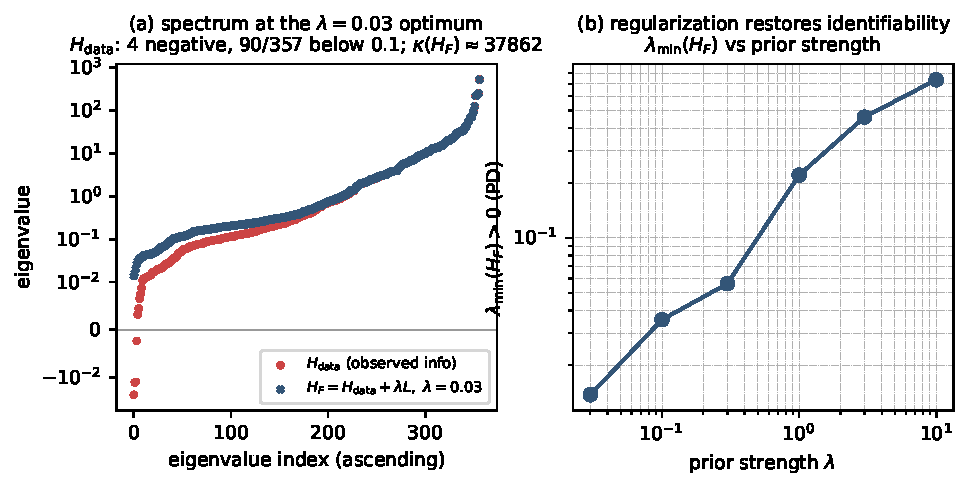
\includegraphics[width=\linewidth]{fig_s53_spectrum.pdf}\\[3pt]
  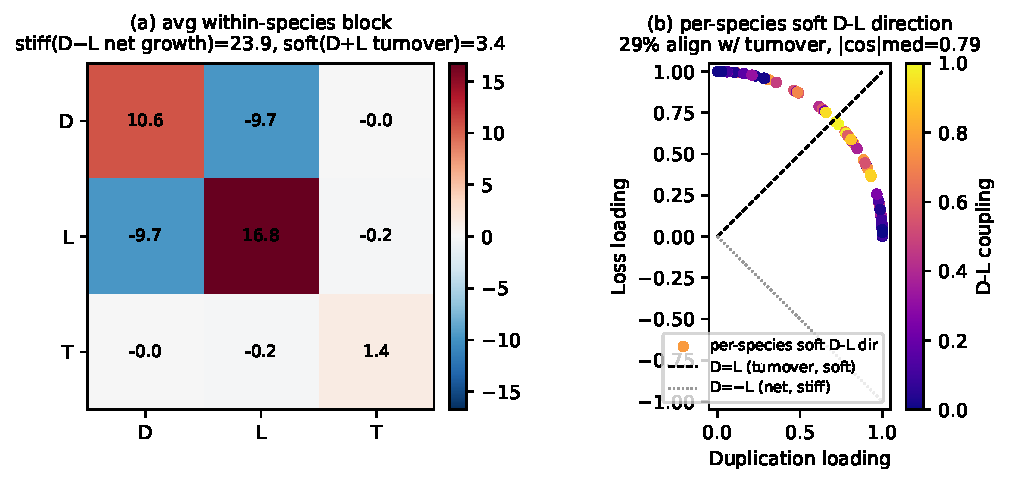
\includegraphics[width=\linewidth]{fig_s53_dl_confounding.pdf}
  \caption{Observed-information analysis at an archaeal species-wise optimum
  ($256$ families, fp64-certified; $p=3S=357$, exact dense $\Fish_{\mathrm{obs}}$).
  \textbf{Top:}
  (left) the data Hessian $\Fish_{\mathrm{obs}}=\Hess_{\mathrm{data}}$ is
  \emph{indefinite} --- $4$ negative eigenvalues and $90/357$ ($25\%$) below
  $0.1$ --- so a quarter of directions are unconstrained by the data alone; the
  GBM prior $\lambda L$ lifts them to make $\Hess_F=\Hess_{\mathrm{data}}+\lambda L$
  positive definite. (right) $\lambda_{\min}(\Hess_F)$ climbs monotonically with
  prior strength ($0.014\!\to\!0.74$ over $\lambda=0.03\!\to\!10$): regularization
  restores identifiability. \textbf{Bottom:} (left) the average within-species
  $3\times3$ block diagonalizes to a \emph{stiff} net-growth axis $\bdelta-\blambda$
  (eig $23.9$) and a \emph{soft} turnover axis $\bdelta+\blambda$ (eig $3.4$);
  transfer is decoupled. (right) per species, the soft duplication--loss direction
  (coloured by D--L coupling) clusters on the turnover diagonal $\bdelta=\blambda$
  --- strongly-coupled species sit exactly on it.}
  \label{fig:fisher}
\end{figure}

\begin{figure}[t]\centering
  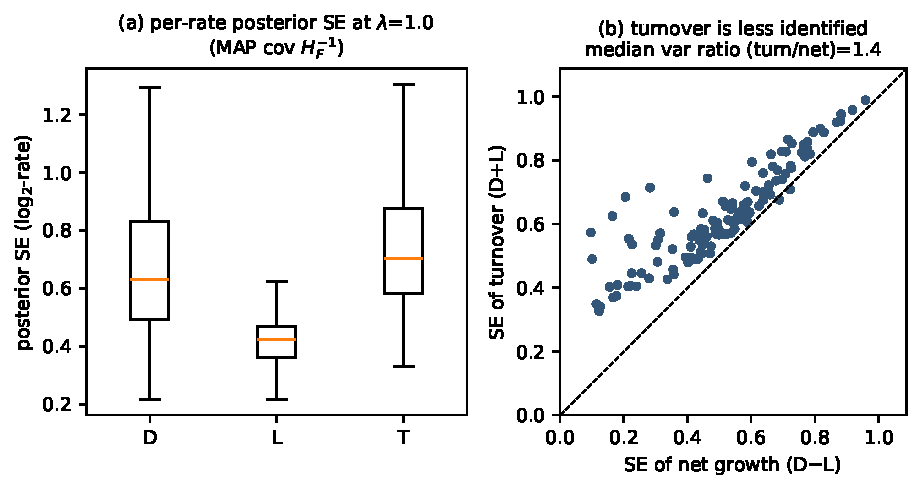
\includegraphics[width=\linewidth]{fig_s53_se.pdf}
  \caption{Asymptotic uncertainty from $\Fish_F^{-1}$ at the cross-validated
  optimum ($\lambda=1$, where $\Hess_F\succ0$). (left) per-rate posterior standard
  errors (log$_2$-rate): median $\bdelta\!=\!0.63$, $\blambda\!=\!0.42$,
  $\btau\!=\!0.70$ ($95\%$ CI factors $\times/\,2.35,\,1.78,\,2.60$). Transfer,
  though decoupled, carries the \emph{largest} SE --- it is identifiable but only
  gently determined. (right) the turnover combination $\bdelta+\blambda$ has
  $1.4\times$ the posterior variance of net growth $\bdelta-\blambda$ for
  \emph{every} species: turnover is the least-identified direction even after
  regularization.}
  \label{fig:fisher-se}
\end{figure}

% ----------------------------------------------------------
\subsection{Transfer heterogeneity via per-recipient weights}
\label{sec:receiver}
\begin{expbox}{Receiver weights}
Fit the model with and without per-recipient weights $w$. (a) Show that the
inferred $w_s$ identify species/lineages that disproportionately receive
transfers, and relate them to known biology where possible. (b) Compare model
fit (held-out likelihood and/or information criterion) with vs.\ without
$w$, controlling for the added parameters. \emph{Goal:} show \toolname can
express and infer across-species transfer heterogeneity --- a model extension
listed as future work for \textsc{AleRax} --- at no additional derivation cost.
\end{expbox}

% ----------------------------------------------------------
\subsection{Custom penalty + cross-validation on \textsc{Hogenom} (the GPU-enabled study)}
\label{sec:cv}
\begin{expbox}{Cross-validated tree-smoothing prior}
Fit \emph{species-wise} DTL rates on \textsc{Hogenom} with the tree-smoothing
prior of Eq.~\eqref{eq:gbm}. Select the penalty strength $\kappa$ by $K$-fold
cross-validation over gene families: for each $\kappa$ on a grid and each fold,
fit on the training families and evaluate the held-out negative log-likelihood.
Report (a) the CV curve (held-out NLL vs.\ $\kappa$) with the selected
$\kappa^\star$; (b) evidence that regularization \emph{improves} held-out
likelihood relative to the unpenalized MLE and reduces degenerate
(boundary-saturated / non-identifiable) estimates; (c) the total compute
($\#\kappa \times K$ full fits) and wall-clock, contrasted with an estimate of
the CPU time the same protocol would require. \emph{Goal:} demonstrate a
statistically principled, cross-validated model-selection workflow for DTL
rates that is \emph{enabled by GPU throughput} and would be impractical on the
CPU --- the headline ``only-possible-because-differentiable-and-fast'' result.
\end{expbox}

\paragraph{Cross-validation selects a regularizing prior.} On $1{,}055$
\textsc{Hogenom} families with $K{=}5$-fold cross-validation over a grid of
$\kappa$, the tree-smoothing prior of Eq.~\eqref{eq:gbm} improves held-out
likelihood over the unpenalized MLE and selects $\kappa^\star\!\approx\!1$. At
$\kappa^\star$ the fraction of boundary-saturated species-wise rates falls from
$\approx\!0.64$ (unpenalized) to $\approx\!0.05$, and --- unlike the
lightly-penalized $\kappa{=}0.03$ fit of Sec.~\ref{sec:certify} --- the
\emph{unconstrained} optimum is already positive-definite
($\lambda_{\min}=+0.22$): the prior, not a box, supplies the missing
identifiability. The entire sweep ($\#\kappa\times K$ full certified fits) runs
end-to-end on a single GPU, which is what makes the protocol practical.

\begin{figure}[t]\centering
  \fbox{\parbox[c][3.2cm][c]{0.7\linewidth}{\centering \TODO{Fig.\ 2:
  held-out NLL vs.\ penalty strength $\kappa$ (CV curve), $\kappa^\star$ marked.}}}
  \caption{Cross-validated selection of the tree-smoothing penalty for
  species-wise rates on \textsc{Hogenom}. \TODO{caption.}}
  \label{fig:cv}
\end{figure}

% ----------------------------------------------------------
\subsection{Ablation: which extension matters?}
\label{sec:ablation}
\begin{expbox}{Component ablation}
Isolate the contribution of each model extension by held-out likelihood
(cross-validated, same protocol as Sec.~\ref{sec:cv}), filling
Table~\ref{tab:ablation}. \emph{Goal:} clarify how much the tree-smoothing prior
and the transfer weights each contribute, and whether they are complementary.
\end{expbox}
\begin{table}[t]\centering
\caption{Ablation of model extensions (lower held-out NLL is better).
\TODO{fill in; cross-validated, \textsc{Hogenom} species-wise.}}
\label{tab:ablation}
\begin{tabular}{lc}
\toprule
Model & Held-out NLL \\
\midrule
Baseline DTL (MLE)              & \TODO{} \\
\;+ tree-smoothing prior        & \TODO{} \\
\;+ transfer weights            & \TODO{} \\
\;+ smoothing + transfer weights & \TODO{} \\
\bottomrule
\end{tabular}
\end{table}

% =====================================================================
\section{Discussion}
\label{sec:discussion}

\paragraph{An extensible, differentiable engine.} The unifying theme is that a
single design choice --- implementing the reconciliation likelihood as a
differentiable GPU program --- yields speed, second-order inference, and model
flexibility together. New terms (priors, alternative recipient models,
hierarchical rate structure) are written as \textsc{PyTorch} expressions and
require \emph{no} hand-derived gradients or Hessians; they immediately inherit
the optimizer, the HVP-based certification, and the Fisher-information tooling.

\paragraph{Simplicity and reproducibility.} The model can be constructed and
optimized in a few lines in a Jupyter notebook, with direct programmatic access
to the loss, gradient, Hessian--vector product, and per-batch solver controls.
This lowers the barrier to methodological experimentation and makes analyses
reproducible.

\paragraph{From a tool to a platform.} The same differentiable core that gives
the results above also makes several extensions natural rather than bespoke: a
Laplace approximation to the posterior over rates (Bayesian uncertainty without
MCMC), hierarchical priors in which species-wise rates inherit from clade-level
hyperparameters, and the use of differentiable reconciliation as the inner
objective of a species-tree search. We develop these in
Appendix~\ref{app:outlook}; collectively they reframe \toolname as a platform
for model development rather than a single fixed tool.

\paragraph{Limitations.} (i) We address rate estimation and reconciliation
given a fixed species tree and CCP inputs; species-tree search is out of scope
here. (ii) Per-recipient weights and per-species rates add parameters and rely
on the regularization of Sec.~\ref{sec:cv} to remain identifiable. (iii) GPU
memory bounds the largest single batch; we mitigate this with batching and
adaptive solver fidelity. \TODO{revise after experiments.}

% =====================================================================
\section{Conclusion}
\label{sec:conclusion}
We presented \toolname, a GPU-accelerated, differentiable implementation of the
\textsc{UndatedDTL} amalgamated reconciliation likelihood. Beyond an
order-of-magnitude speedup for genewise rate estimation, differentiability
gives certified optima, Fisher-information--based uncertainty and
identifiability analysis, user-defined penalties with cross-validated model
selection, and learned transfer heterogeneity --- capabilities that are
difficult or impossible with existing CPU, first-order tools, and that follow
naturally from exposing reconciliation through a \textsc{PyTorch} interface.

% =====================================================================
\section*{Availability}
\toolname is available at \TODO{repository URL} under \TODO{license}. It installs
as an editable \textsc{PyTorch} package (\texttt{pip install -e .}) plus a
\textsc{Rust} preprocessing extension built with \texttt{cargo build --release};
the resulting shared library is located via the \texttt{GPUREC\_PREPROCESS\_PATH}
environment variable. Every experiment in this paper is reproduced by a single
notebook, \texttt{experiments/sanderson\_cv/reproduce\_experiments.ipynb}, and the
following self-contained drivers, each runnable on one GPU and each writing a
self-describing artifact:
\begin{itemize}[nosep]
\item \textbf{Speed (Sec.~\ref{sec:speed})} --- \texttt{bench\_genewise\_warm\_rebatch.py}:
  per-family rates to $|P\grad|<10^{-3}$ on \textsc{Hogenom}.
\item \textbf{Certified optimum (Sec.~\ref{sec:certify}) and receiver weights
  (Sec.~\ref{sec:receiver})} --- \texttt{converge\_bounded\_joint\_archaea.py}:
  box-constrained joint $(\theta,\alpha)$ Newton--CG with the deflated-gauge
  positive-definiteness certificate and the receiver-weight Fisher information.
\item \textbf{Observed information (Sec.~\ref{sec:fisher})} ---
  \texttt{fisher\_information\_s53.py}: the dense $\Fish_{\mathrm{obs}}$ spectrum,
  the duplication--loss confounding, and asymptotic standard errors.
\item \textbf{Cross-validation (Secs.~\ref{sec:cv} and~\ref{sec:ablation})} ---
  \texttt{run\_cv.py}: $K$-fold tree-smoothing cross-validation over a $\kappa$ grid.
\end{itemize}
Datasets are the published \textsc{Hogenom} and \citet{Davin2018} archaeal CCP
collections (\TODO{data DOI / download}); each driver reads its data root from an
environment variable, and the notebook prints the exact command and expected
numbers for each result.

\section*{Acknowledgements}
\TODO{}

% =====================================================================
\appendix
\section{Extensions and outlook: differentiable reconciliation as a platform}
\label{app:outlook}
The capabilities in the main text all follow from one design choice --- a
differentiable, GPU-resident reconciliation likelihood with exact gradients and
Hessian--vector products. The same machinery makes the following extensions
natural; we sketch them here as the roadmap that distinguishes \toolname from a
single fixed tool. None requires hand-derived derivatives: each is expressed as
a \textsc{PyTorch} term and inherits the optimizer, the matrix-free HVP, and the
information-matrix tooling.

\subsection{Bayesian inference by Laplace approximation}
\label{app:laplace}
Because the Hessian at the MAP/ML estimate is available matrix-free, the
posterior over rates admits a Gaussian (Laplace) approximation
\begin{equation}
  p(\theta \mid D) \;\approx\; \mathcal{N}\!\left(\hat\theta,\; \Hess(\hat\theta)^{-1}\right),
  \label{eq:laplace}
\end{equation}
giving credible intervals and posterior correlations \emph{without} MCMC. The
required linear solves with $\Hess$ reuse the same matrix-free conjugate-gradient
/ Lanczos routines used for optimization and certification; one never forms or
inverts the dense Hessian. This turns the point estimates that current
reconciliation tools report into full uncertainty statements, and enables
penalty-based (marginal-likelihood / information-criterion) model comparison
between the extensions of Sec.~\ref{sec:penalty}--\ref{sec:rweights}.

\subsection{Hierarchical (clade-level) rate priors}
\label{app:hier}
The penalty framework of Sec.~\ref{sec:penalty} generalizes to a hierarchy:
per-species rates $\theta_s$ can be drawn from clade-level hyper-parameters
$\mu_c$ (themselves estimated), e.g.\ $\theta_s \sim \mathcal{N}(\mu_{c(s)},
\sigma^2)$ with the tree-Laplacian (Eq.~\eqref{eq:gbm}) as the special case of a
single global level. This partial pooling shares strength among related lineages
--- regularizing the weakly-identified directions diagnosed in
Sec.~\ref{sec:fisher} --- and is again just an additional differentiable term in
$R(\theta)$, with the hyper-parameters optimized (empirical Bayes) or integrated
(via the Laplace approximation of App.~\ref{app:laplace}).

\subsection{Differentiable reconciliation inside species-tree search}
\label{app:treesearch}
The main text fixes the species tree $S$. Species-tree inference
(\textsc{SpeciesRax}/\textsc{AleRax}) searches over $S$ by SPR moves, recomputing
rates at each candidate. A fast, differentiable rate-estimation inner loop is
exactly the expensive primitive that search repeatedly invokes; \toolname can
serve as that inner objective, and the gradient/curvature it exposes opens the
possibility of continuous relaxations of branch-level structure. We leave a full
treatment to future work, but note that the engine presented here is the
component such a search would be built around.

\subsection{Other consequences}
\label{app:other}
The same interface supports: alternative recipient models beyond the softmax of
Sec.~\ref{sec:rweights} (any differentiable parameterization); gradient-based
sensitivity analysis of inferred DTL event counts to the rates; and integration
with the broader differentiable-programming ecosystem (e.g.\ amortized or
variational inference over rates). Each is a direct consequence of exposing the
likelihood, its gradient, and its curvature through a standard autodiff
interface.

% =====================================================================
\begin{thebibliography}{99}
\small

\bibitem[Morel et~al.(2024)]{Morel2024} Morel B, Williams TA, Stamatakis A, Sz\"oll\H{o}si GJ.
AleRax: a tool for gene and species tree co-estimation and reconciliation under
a probabilistic model of gene duplication, transfer, and loss.
\emph{Bioinformatics} 2024;40(4):btae162.

\bibitem[Morel et~al.(2022)]{Morel2022} Morel B, Schade P, Lutteropp S, et al. SpeciesRax: a tool
for maximum likelihood species tree inference from gene family trees under
duplication, transfer, and loss. \emph{Mol Biol Evol} 2022;39:msab365.

\bibitem[Morel et~al.(2020)]{Morel2020} Morel B, Kozlov AM, Stamatakis A, Sz\"oll\H{o}si GJ.
GeneRax: a tool for species-tree-aware maximum likelihood-based gene family tree
inference under gene duplication, transfer, and loss.
\emph{Mol Biol Evol} 2020;37:2763--2774.

\bibitem[Sz\"oll\H{o}si et~al.(2013)]{Szollosi2013} Sz\"oll\H{o}si GJ, Rosikiewicz W, Boussau B, et al.
Efficient exploration of the space of reconciled gene trees.
\emph{Syst Biol} 2013;62:901--912.

\bibitem[Sz\"oll\H{o}si et~al.(2015)]{Szollosi2015} Sz\"oll\H{o}si GJ, Tannier E, Daubin V, Boussau B. The
inference of gene trees with species trees. \emph{Syst Biol} 2015;64:e42--e62.

\bibitem[H\"ohna and Drummond(2012)]{Hohna2012} H\"ohna S, Drummond AJ. Guided tree topology proposals for
Bayesian phylogenetic inference. \emph{Syst Biol} 2012;61:1--11.

\bibitem[Larget(2013)]{Larget2013} Larget B. The estimation of tree posterior probabilities
using conditional clade probability distributions.
\emph{Syst Biol} 2013;62:501--511.

\bibitem[Sanderson(2002)]{Sanderson2002} Sanderson MJ. Estimating absolute rates of molecular
evolution and divergence times: a penalized likelihood approach.
\emph{Mol Biol Evol} 2002;19:101--109.

\bibitem[Penel et~al.(2009)]{Penel2009} Penel S, Arigon A-M, Dufayard J-F, et al. Databases of
homologous gene families for comparative genomics.
\emph{BMC Bioinformatics} 2009;10:S3.

\bibitem[Williams et~al.(2017)]{Williams2017} Williams TA, Sz\"oll\H{o}si GJ, Spang A, et al.
Integrative modeling of gene and genome evolution roots the archaeal tree of
life. \emph{Proc Natl Acad Sci USA} 2017;114:E4602--E4611.

\bibitem[Dav\'in et~al.(2018)]{Davin2018} Dav\'in AA, Tannier E, Williams TA, et al. Gene transfers
can date the tree of life. \emph{Nat Ecol Evol} 2018;2:904--909.

\bibitem[Felsenstein(1988)]{Felsenstein1988} Felsenstein J. Phylogenies from molecular sequences:
inference and reliability. \emph{Annu Rev Genet} 1988;22:521--565.

\bibitem[Zhang and Mirarab(2022)]{Zhang2022} Zhang C, Mirarab S. ASTRAL-Pro 2: ultrafast species tree
reconstruction from multi-copy gene family trees.
\emph{Bioinformatics} 2022;38:4949--4950.

\bibitem[Paszke et~al.(2019)]{Paszke2019} Paszke A, Gross S, Massa F, et al. PyTorch: an imperative
style, high-performance deep learning library. \emph{NeurIPS} 2019.

\bibitem[Kingma and Ba(2015)]{Kingma2015} Kingma DP, Ba J. Adam: a method for stochastic
optimization. \emph{ICLR} 2015.

\bibitem[Liu and Nocedal(1989)]{LiuNocedal1989} Liu DC, Nocedal J. On the limited memory BFGS method
for large scale optimization. \emph{Math Program} 1989;45:503--528.

\bibitem[Lanczos(1950)]{Lanczos1950} Lanczos C. An iteration method for the solution of the
eigenvalue problem of linear differential and integral operators.
\emph{J Res Natl Bur Stand} 1950;45:255--282.

\end{thebibliography}

\end{document}
